\documentclass{beamer}

\mode<presentation>
{
  \usetheme{Warsaw}
  % or ...

  \setbeamercovered{transparent}
  % or whatever (possibly just delete it)
}


\usepackage[english]{babel}
\usepackage[utf8]{inputenc}
\usepackage{times}
\usepackage[T1]{fontenc}
\usepackage{graphicx}
\graphicspath{ {images/} }


\title[]
{Implementacja wydajnego wzorca wstrzykiwania zależności dla złożonych grafów zależności}

\author[Adrian Mularczyk]
{Adrian Mularczyk}


\institute[Uniwersytet Wrocławski]
{
Uniwersytet Wrocławski\\
Wydział Matematyki i Informatyki\\
Kierunek: Informatyka
}

\date{}

% Delete this, if you do not want the table of contents to pop up at
% the beginning of each subsection:
%\AtBeginSubsection[]
%{
  %\begin{frame}<beamer>{Outline}
    %\tableofcontents[currentsection,currentsubsection]
  %\end{frame}
%}

\begin{document}

\begin{frame}
  \titlepage
\end{frame}

\begin{frame}{Agenda}
  \tableofcontents
\end{frame}



\section{Przedstawienie problemu}

\subsection*{SOLID}

\begin{frame}{SOLID}
%Na przestrzeni lat powstało bardzo dużo projektów. Część z nich była łatwiejsza w utrzymaniu, część trudniejsza. Analiza tych projektów pozwoliła zauważyć, że są pewne zasady, które powodują, że projekty rozwija się łatwiej. Te zasady zostały połączone w zbiory zasad. Najbardziej popularnych i powszechnie stosowanym zbiorem zasad jest SOLID
\begin{itemize}
	\item S - SRP (Single responsibility principle)
	\item O - OCP (Open/closed principle)
	\item L - LSP (Liskov substitution principle)
	\item I - ISP (Interface segregation principle)
	\item D - DIP (Dependency inversion principle)
\end{itemize}
%Niniejsza praca w dużej mierze skupia się na rozwiązaniu dla zasady DIP - Dependency inversion principle. 
\end{frame}

\begin{frame}{Dependency Inversion Principal}
Wysokopoziomowe moduły nie powinny zależeć od modułów niskopoziomowych. Zależności między nimi powinny wynikać z abstrakcji.
\end{frame}


\subsection*{Kontenery wstrzykiwania zależności}

\begin{frame}{Kontenery wstrzykiwania zależności}
%Aby łatwiej zastosować zasadę DIP można wesprzeć się tzw. kontenerem wstrzykiwania zależności (ang. Dependency Injection Container). 
Obiekt, który przechowuje mapę, w której abstrakcje (interfejsy, klasy abstrakcyjne) mają przyporządkowane implementacje (klasy implementujące interfejsy lub dziedziczące z klas abstrakcyjnych).
\end{frame}

\begin{frame}{Kontenery wstrzykiwania zależności}
%Kontenery dostarczają nam kilku funkcjonalności. Jedną z nich jest możliwość zdefiniowania tego jakiej instancję jakiej klasy należy zwrócić w miejsce konkretnego interfejsu. Drugą jest tworzenie (na podstawie przechowywanego mapowania) instancji obiektów konkretnej klasy lub implementujących określony interfejs.
\begin{itemize}
	\item Rejestracja
	\item Tworzenie obiektów
\end{itemize}
\end{frame}

\subsection*{Problem}

\begin{frame}{Problem}
  \begin{itemize}
  \item
  	W grafach zależności często powtarzają się typy
  \item
  	Utworzenie instancji nowego obiektu zajmuje czas.
  \item
  	Nowe obiekty są często tworzone
  \end{itemize}
\end{frame}

\subsection*{Cel Pracy}

\begin{frame}{Cel Pracy}
Stworzenie wydajenego kontenera wstrzykiwania zależności, który będzie wydajny dla zlożonych grafów zależności, a także który będzie efektywnie tworzył kolejne instancje tej samej klasy.
\end{frame}


\section{Wstrzykiwanie zależności}

\subsection*{Rodzaje wstrzykiwań zależności}

\begin{frame}{Rodzaje wstrzykiwań zależności}
%Wstrzykiwanie zależności jest niczym więcej niż techniką, która umożliwia luźne powiązania, a luźne powiązania sprawiają, że kod jest rozszerzalny i łatwy w utrzymaniu.
%Wstrzykiwanie zależności może odbywać się na 3 sposoby:
\begin{itemize}
	\item Wstrzykiwanie przez konstruktor.
	\item Wstrzykiwanie przez metodę.
	\item Wstrzykiwanie przez właściwość.
\end{itemize}
\end{frame}


\subsection*{Implementacje przemysłowe}

\begin{frame}{Implementacje przemysłowe}
%Na rynku jest wiele implementacji wstrzykiwania zależności. Poniżej przedstawiono kilka najbardziej popularnych (według ilości pobrań z NuGet) oraz kilka najszybszych (według rankingu na blogu Daniela Palme)
\begin{itemize}
	\item Unity
	\item NInject
	\item Autofac
	\item StructureMap
	\item Windsor
	\item Grace
	\item DryIoc
	\item LightInject
	\item SimpleInjector
\end{itemize}
\end{frame}



\section{Implementacja}
%Na początku chciałbym pokrótce opisać dwie rzeczy, które są istotne dla rozwiązania przedstawionego w niniejszej pracy. Pierwszą z nich jest \textbf{Common Intermediate Language}, a drugą przestrzeń nazw \textbf{Reflection.Emit}.
\begin{frame}{Implementacja}
\begin{itemize}
	\item CIL
	\item Reflection.Emit
\end{itemize}
%CIL to skrót od Common Intermediate Language. Jest to język pośredni do którego jest kompilowany kod C\#. Język ten pozwala na komunikację między aplikacjami napisanymi na platformie .NET, a systemem operacyjnym. CIL jest językiem w całości opartym na stosie.
%Dodatkowo jest w nim możliwość zdefiniowania zmiennych lokalnych, a także wczytania argumentów. Dostępnymi operacjami są: pobranie wartości ze stosu, umieszczenie wartości na stosie, operacje arytmetyczne oraz wywołanie funkcji.
%Przestrzeń nazw \textbf{Reflection.Emit} pozwala w kodzie programu, w sposób dynamiczny, na utworzenie listy operacji w języku CIL, a następnie zapamiętanie ciągu tych operacji jako delegat. Za każdym razem, gdy delegat zostanie wywołany, wykona się ciąg wcześniej zdefiniowanych operacji CIL.
\end{frame}

\subsection*{Dwa rozwiązania}

\begin{frame}{Dwa rozwiązania}
%Pomysł był taki, aby wykorzystać Reflection.Emit do utworzenia listę operacji w języku CIL, która dla danego typu, zwróci nam obiekt tego typu.
%Ten pomysł został zrealizowany na dwa sposóby:
\begin{itemize}
	\item Partial Emit Function
	\item Full Emit Function
\end{itemize}
%W obu rozwiązaniach metoda do rejestracji wygląda tak samo. Różnią się one jedynie tym jak nowy obiekt jest tworzony.
\end{frame}


\subsection*{Partial Emit Function}

\begin{frame}{Partial Emit Function}
%Ten algorytm działa rekurencyjnie. Dla danego typu najpierw tworzone są obiekty, które są wymagane przez konsruktor, a następnie nowy obiekt jest tworzony z wykorzystaniem wcześniej utworzonych typów. Metoda ta została nazwana Partial, ponieważ obiekt jest tworzony częściowo, kawałek po kawałku.
%Każda z takich części wykorzystuje Reflecion.Emit do stworzenia delegata, który jako argument przyjmuje listę obiektów wymaganych przez konstruktor, a następnie przy użyciu danego konstruktora i listy obiektów tworzny nowy obiekt.
<jakiś rysunek że z kawałku tworzy się co nowego>
\end{frame}


\subsection*{Full Emit Function}

\begin{frame}{Full Emit Function}
%Ten algorytm tworzy jedną dużą listę operacji CIL, która zawiera tworzenie wszystkich pośrednich obiektów oraz tworzenie głównego obiektu.
<jakiś rysunek że jest jeden duży kawałek>
%Jak pokazują wyniki czasem bardziej opłąca się używać pierwszej motody, a czasem drugiej.
\end{frame}




\section{Wyniki}
%W testach chciałem się przekonać, czy faktycznie zaprezentowane przeze mnie rozwiązanie jest wydajne.

\subsection*{Przypadek testowy A}

\begin{frame}{Przypadek testowy A - graf zależności}
\begin{figure}[H]
	\begin{center}
  		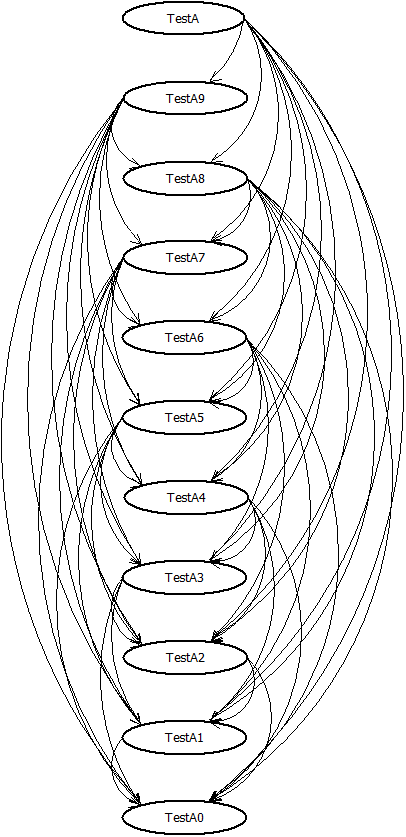
\includegraphics[height=6cm]{TestA.png}
	\end{center}
\end{figure}
\end{frame}

\begin{frame}{Przypadek testowy A - Transient}
Liczba iteracji: 1 i 10
\begin{table}
\begin{small}
	\begin{tabular}{ l  r }
		\begin{tabular}{ | l | r | }
    		\hline
		Autofac &  0 \\ \hline
		\textbf{NiquIoCPartial}  & \textbf{1} \\ \hline
		Windsor & 1 \\ \hline
		\textbf{NiquIoCFull} & \textbf{8} \\ \hline
		Unity & 8 \\ \hline
		LightInject & 10 \\ \hline
		StructureMap & 10 \\ \hline
		Ninject & 11 \\ \hline
		SimpleInjector & 13 \\ \hline
		DryIoc & 14 \\ \hline
		Grace & 15 \\ \hline
  		\end{tabular}
	&
		\begin{tabular}{ | l | r | }
    		\hline
		\textbf{NiquIoCPartial} & \textbf{3} \\ \hline
		Autofac & 6 \\ \hline
		\textbf{NiquIoCFull} & \textbf{8} \\ \hline
		LightInject & 10 \\ \hline
		SimpleInjector & 14 \\ \hline
		StructureMap & 14 \\ \hline
		DryIoc & 15 \\ \hline
		Grace & 16 \\ \hline
		Unity & 16 \\ \hline
		Windsor & 16 \\ \hline
		Ninject & 90 \\ \hline
  		\end{tabular}
  	\end{tabular}
\end{small}
\end{table}
\end{frame}


\begin{frame}{Przypadek testowy A - Transient}
Liczba iteracji: 100 i 1000
\begin{table}
\begin{small}
	\begin{tabular}{ l  r }
		\begin{tabular}{ | l | r | }
    		\hline
		\textbf{NiquIoCFull} & \textbf{9} \\ \hline
		LightInject & 11 \\ \hline
		SimpleInjector & 15 \\ \hline
		DryIoc & 16 \\ \hline
		Grace & 18 \\ \hline
		\textbf{NiquIoCPartial} & \textbf{19} \\ \hline
		StructureMap & 54 \\ \hline
		Autofac & 59 \\ \hline
		Unity & 88 \\ \hline
		Windsor & 155 \\ \hline
		Ninject & 882 \\ \hline
  		\end{tabular}
	&
		\begin{tabular}{ | l | r | }
    		\hline
		\textbf{NiquIoCFull} & \textbf{18} \\ \hline
		LightInject & 19 \\ \hline
		SimpleInjector & 29 \\ \hline
		DryIoc & 29 \\ \hline
		Grace & 37 \\ \hline
		\textbf{NiquIoCPartial} & \textbf{173} \\ \hline
		StructureMap & 417 \\ \hline
		Autofac & 587 \\ \hline
		Unity & 813 \\ \hline
		Windsor & 1529 \\ \hline
		Ninject & 8934 \\ \hline
  		\end{tabular}
  	\end{tabular}
\end{small}
\end{table}
\end{frame}


\subsection*{Przypadek testowy C}

\begin{frame}{Przypadek testowy C - graf zależności}
\begin{figure}[H]
	\begin{center}
  		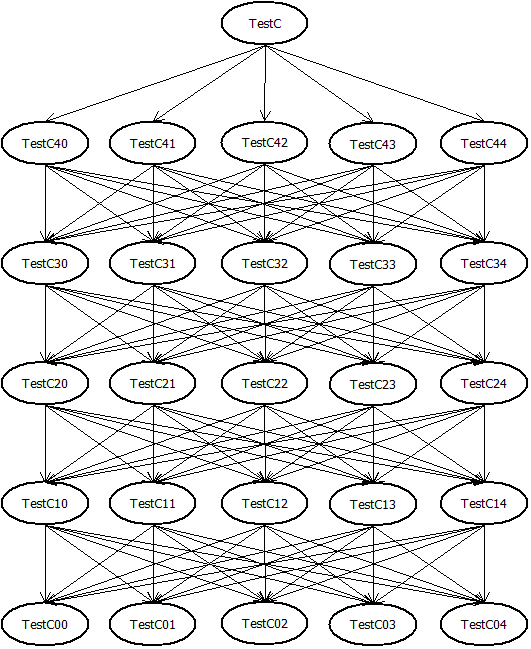
\includegraphics[height=6cm]{TestC.png}
	\end{center}
\end{figure}
\end{frame}

\begin{frame}{Przypadek testowy C - Transient}
Liczba iteracji: 1 i 10
\begin{table}
\begin{small}
	\begin{tabular}{ l  r }
		\begin{tabular}{ | l | r | }
    		\hline
		Autofac &  0 \\ \hline
		\textbf{NiquIoCPartial}  & \textbf{1} \\ \hline
		Windsor & 1 \\ \hline
		\textbf{NiquIoCFull} & \textbf{8} \\ \hline
		Unity & 8 \\ \hline
		LightInject & 10 \\ \hline
		StructureMap & 10 \\ \hline
		Ninject & 11 \\ \hline
		SimpleInjector & 13 \\ \hline
		DryIoc & 14 \\ \hline
		Grace & 15 \\ \hline
  		\end{tabular}
	&
		\begin{tabular}{ | l | r | }
    		\hline
		\textbf{NiquIoCPartial} & \textbf{3} \\ \hline
		Autofac & 6 \\ \hline
		\textbf{NiquIoCFull} & \textbf{8} \\ \hline
		LightInject & 10 \\ \hline
		SimpleInjector & 14 \\ \hline
		StructureMap & 14 \\ \hline
		DryIoc & 15 \\ \hline
		Grace & 16 \\ \hline
		Unity & 16 \\ \hline
		Windsor & 16 \\ \hline
		Ninject & 90 \\ \hline
  		\end{tabular}
  	\end{tabular}
\end{small}
\end{table}
\end{frame}


\begin{frame}{Przypadek testowy C - Transient}
Liczba iteracji: 100 i 1000
\begin{table}
\begin{small}
	\begin{tabular}{ l  r }
		\begin{tabular}{ | l | r | }
    		\hline
		\textbf{NiquIoCFull} & \textbf{9} \\ \hline
		LightInject & 11 \\ \hline
		SimpleInjector & 15 \\ \hline
		DryIoc & 16 \\ \hline
		Grace & 18 \\ \hline
		\textbf{NiquIoCPartial} & \textbf{19} \\ \hline
		StructureMap & 54 \\ \hline
		Autofac & 59 \\ \hline
		Unity & 88 \\ \hline
		Windsor & 155 \\ \hline
		Ninject & 882 \\ \hline
  		\end{tabular}
	&
		\begin{tabular}{ | l | r | }
    		\hline
		\textbf{NiquIoCFull} & \textbf{18} \\ \hline
		LightInject & 19 \\ \hline
		SimpleInjector & 29 \\ \hline
		DryIoc & 29 \\ \hline
		Grace & 37 \\ \hline
		\textbf{NiquIoCPartial} & \textbf{173} \\ \hline
		StructureMap & 417 \\ \hline
		Autofac & 587 \\ \hline
		Unity & 813 \\ \hline
		Windsor & 1529 \\ \hline
		Ninject & 8934 \\ \hline
  		\end{tabular}
  	\end{tabular}
\end{small}
\end{table}
\end{frame}


\section{Podsumowanie}

\begin{frame}{Podsumowanie}
%Zaproponowane rozwiązania bardzo dobrze realizują postawione we wstępie pracy cele. Dla wszystkich przypadków testowych, dla każdego z rodzaju rejestracji, jedno z przedstawionych rozwiązań osiągało najlepsze wyniki albo odbiegały one niewiele od najlepszych wyników. Zawsze któreś z przedstawionych rozwiązań było w pierwszej trójce rozwiązań z najlepszymi czasami, a czasami nawet oba. Możliwość mieszania użyć zaprezentowanych rozwiązań (w jednym projekcie można korzystać z obu rozwiązań niezależnie) sprawia, że \textbf{NiquIoC} jest najbardziej wydajną implementacją wzorca wstrzykiwania zależności dla złożonych grafów zależności.
\end{frame}

\end{document}


